\documentclass[a4paper]{article}

\usepackage[utf8]{inputenc}
\usepackage{chngpage}
\usepackage{wrapfig}
\usepackage[T1]{fontenc}
\usepackage{textcomp}
\usepackage{listings}
\usepackage{lmodern}
\usepackage{amsfonts}
\usepackage{lipsum}
\usepackage[left=0.67in, right=0.67in, bottom=0.67in, top=0.67in]{geometry}
\usepackage{amsthm}
\usepackage{tcolorbox}
\usepackage{relsize}
\usepackage{titlesec}
\usepackage{makecell}
\usepackage{titletoc}
\usepackage{hyperref}
\usepackage{xcolor}
\usepackage{colortbl}
\usepackage{tabularx}
\usepackage{graphicx}
\usepackage{makeidx}
\usepackage{tikz}
\usepackage{cases}
\usepackage{svg}
\usepackage{apacite}
\usepackage{tkz-berge}
\usepackage{url}
\usepackage{tgtermes}
\usepackage{sectsty}
\usepackage{subcaption}
\usepackage{setspace}
\usepackage{float}
\usepackage{multirow}
\usepackage{amsmath, amssymb}


% figure support
\usepackage{import}
\usepackage{xifthen}
\pdfminorversion=7
\usepackage{pdfpages}
\usepackage{transparent}
\usepackage{color}
\newcommand{\incfig}[2][1]{%
    \def\svgwidth{#1\columnwidth}
    \import{./figures/}{#2.pdf_tex}
}

%mathstyling
\theoremstyle{plain}
\newtheorem{thm}{Theorem}[section]
\newtheorem{lem}[thm]{Lemma}
\newtheorem{prop}[thm]{Proposition}
\newtheorem*{cor}{Corollary}

\theoremstyle{definition}
\newtheorem{defn}{Definition}[section]
\newtheorem{conj}{Conjecture}[section]
\newtheorem{exmp}{Example}[section]
\newtheorem{axiom}{Axiom}
\theoremstyle{remark}
\newtheorem*{rem}{Remark}
\newtheorem*{note}{Note}

\definecolor{darkgreen}{rgb}{0.0, 0.5, 0.0}

\pdfsuppresswarningpagegroup=1
\lstset{
tabsize = 4, %% set tab space width
showstringspaces = false, %% prevent space marking in strings, string is defined as the text that is generally printed directly to the console
numbers = left, %% display line numbers on the left
commentstyle = \color{darkgreen}, %% set comment color
keywordstyle = \color{blue}, %% set keyword color
stringstyle = \color{red}, %% set string color
rulecolor = \color{black}, %% set frame color to avoid being affected by text color
basicstyle = \small \ttfamily , %% set listing font and size
breaklines = true, %% enable line breaking
numberstyle = \tiny,
  frame=none,
  xleftmargin=2pt,
  stepnumber=1,
  belowcaptionskip=\bigskipamount,
  captionpos=b,
  escapeinside={*'}{'*},
  language=haskell,
  tabsize=2,
  emphstyle={\bf},
  showspaces=false,
  columns=flexible,
  showstringspaces=false,
  morecomment=[l]\%,
}
\begin{document}
\hline
\begin{center}
	\vspace{1mm}
	\Huge CS261: Planning $\&$ Design Report
\end{center}
\hline
\section*{Technical Description}
\subsection*{Purpose of the Program}
Our software will allow a user to track the software development project they are managing and also creates a risk assessment (initial and as the project progresses) which is evaluated using several metrics (hard and soft). Risky areas and suggestions on how to mitigate these risks for any software project will also be highlighted. This will be done through a website which can be accessed by the project leader. This design document illustrates the preliminary planning and design of our software. We will provide a description of processes to give an idea of how our software will work along with justification for our design choices. An outline of the user interface, subsystems interaction, testing plans and also risk assessments will be covered. Naturally, some specifics of the final product may differ from what is described but the general architecture and design should be similar.
\subsection*{Language and Libraries}
Our choice of language was primarily motivated by our team’s familiarity with Python and web technologies (Javascript, HTML/CSS), the compatibility between these languages, and appropriate libraries. Additionally, Python is a typical choice for ML applications, and we will be using SQLite for its interoperability with web libraries. The libraries are as follows:
		\begin{itemize}
			\item \textbf{Flask} - web development library made for Python 3.
			\item \textbf{WTForms} - created with compatibility with Flask in mind, this library makes creating web forms significantly easier if they include specific validators.
			\item \textbf{SQLAlchemy} - database object relational mapper, that is, databases can be expressed as objects in Python 3.
			\item \textbf{Werkzeug} - security library used for things such as password hashing.
			\item \textbf{PyGithub} - allows our project to retrieve GitHub repository data. Used as a metric.
			\item \textbf{sklearn} - Machine learning classification and regression toolkit library. 
			\item \textbf{Pyfpdf} - PDF generation library. Will be primarily used to create the project risk and data graph output.
			\item \textbf{Matplotlib} - Library that is used to generate graphs to present data to the manager.
		\end{itemize}
\section*{Description of Processes}
\subsection*{Database Schema}
\begin{figure}[H]
	\centering
	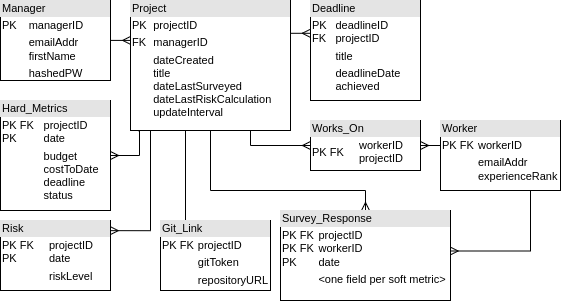
\includegraphics[width=0.65\textwidth]{tables.png}
	\caption{Database Schema}
	\label{fig:tables-png}
\end{figure}
\noindent \textbf{Manager Table}
The manager table is accountable for keeping manager accounts registered within our system. All passwords are hashed for security. \\

\noindent\textbf{Project Table}\\
This table is created if a manager creates a new project. Each project is associated with its creator, the manager, thus the foreign key is the managerID. Every project has an updateInterval that stores the frequency of our emailed surveys and the frequency of GitHub pushes within that interval.  dateLastSurveyed and dateLastRiskCalculation are stored to enable periodic pushes of the survey and updates to risk calculation respectively. \\

\noindent\textbf{Hard$\_$Metric Table}\\
The hard metric table stores all initial hard metrics after the creation of a new project. Creating a separate table for hard metrics allows our system to update and create new rows easier when implementing the form within our website. Furthermore, the separation makes it easy to implement new hard metrics in case of an update in the future.\\

\noindent\textbf{Risk Table} \\
The Risk table stores the calculated risk from our algorithm and associates it with a project, along with its date of calculation to track dateLastRiskCalculation in the Project table. \\

\noindent\textbf{Git$\_$Link Table}\\
This table was chosen to be separate as gitToken, the GitHub token, can expire and be changed. Separating the table makes pushing the form easier. ProjectID was chosen to be the primary and foreign key to create a one-to-one relationship with Project table. \\

\noindent\textbf{Deadline Table}\\
This table stores the internal deadlines of a project that the manager creates. Each deadline is represented as a row. \\

\noindent\textbf{Worker Table}\\
This table stores all the software engineers that are associated with our system. Note that experience can vary from the same software engineer depending on their role. As such, the primary key is the workerID instead of the emailAddr, allowing them to change the experienceRank depending on the project. \\

\noindent \textbf{Works$\_$On Table} \\
The Works$\_$On table links the Worker Table with the Project Table.
\subsection*{Use-Case, Sequence Diagrams and Interaction}
We have designed a Use-Case diagram to present all possible actions of key actors in our system, represented by figure \ref{fig:usecase} below. Note that the actions available depend not only on the role of the user (Manager/Developer) but also on whether they are signed-in or not.\\
The interaction of our system is as follows:\\

\noindent\textbf{Log-in/Sign-up} \\
A manager logs in or signs up using the login/signup form of our website. A signup would create a new row in the table Managers, whereas a login would check for existing credentials in the table. There is no interaction with the algorithm in this functionality. \\

\noindent \textbf{Project creation}\\
See figure \ref{sequence}. \\

\noindent\textbf{Editing project data}\\
Editing project data, such as its existing hard metrics, is similarly explained in figure \ref{sequence}. In particular, once hard metrics are POSTed through the website, a new row in the Hard$\_$Metric table is inserted with data. This data is then fetched by the algorithm to re-calculate the risk. After the re-calculation, the new risk is stored in the Risk table and can be displayed in the website at will. \\

\noindent \textbf{Survey}\\
The survey interaction of our system is split into an if statement. If the software engineer fills the survey for the first time, the website prompts an initial survey. Once the initial survey is filled into the website and stored in the database, the website prompts back to the software engineer with the soft metric survey. Once the soft metric survey data is POSTed, this data is stored in the database under the Survey$\_$Response table. This data is then fed into the algorithm, which re-calculates the risk, stores it in the database, which then can be viewed by the manager. If it is not the first time, the steps explained above repeat, except that they do not fill in the initial survey.
\begin{figure}[H]
    \centering
    \begin{minipage}{0.5\textwidth}
        \centering
        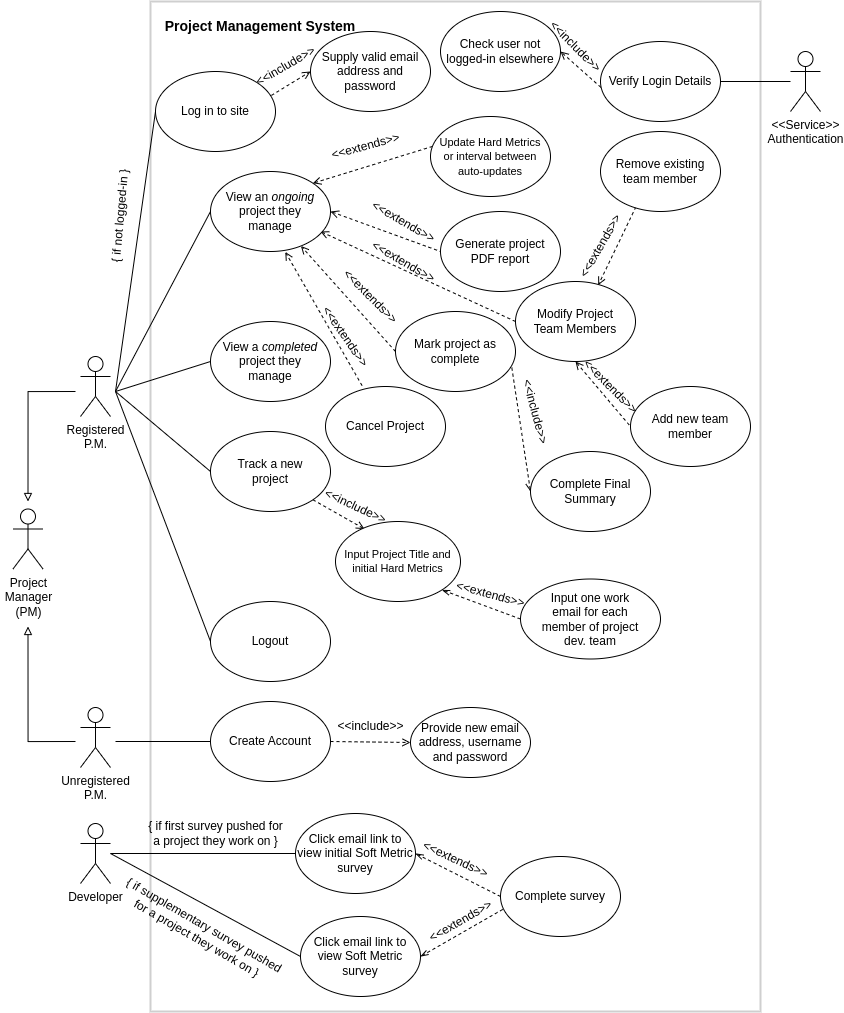
\includegraphics[width=1\textwidth]{usecase.png} % first figure itself
        \caption{Use-Case diagram of our system}
	\label{fig:usecase}
    \end{minipage}\hfill
    \begin{minipage}{0.5\textwidth}
        \centering
        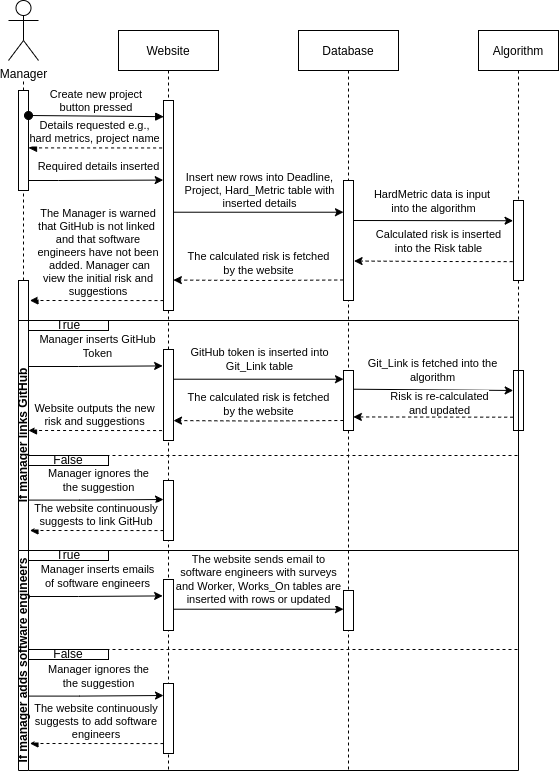
\includegraphics[width=1\textwidth]{sequence.png} % second figure itself
        \caption{Sequence diagram of creating a project}
	\label{sequence}
    \end{minipage}
\end{figure}
\subsection*{Risk Assessment Model}
The role of the Risk-Assessment Model is to receive a snapshot of the project metrics at a specific point in the development (the independent variables) and to return a value indicating whether the project is likely to be a success or a failure (the dependent variable). Given the complexity of such a relationship, we decided it would be most effective to use a form of Supervised Learning, where the model is trained on labelled data (I.e. a set of projects at various points in their development which have been labelled as ultimately being a success or failure). Furthermore, each project which is tracked to completion/failure using the software provides a new row of training data which can be fed-back into the learning model, to improve the accuracy over-time.\\
 
\noindent For this problem, there are two main types of Machine Learning model which are applicable: Classification and Regression. Initially, we planned to implement a Classifier such as Support Vector Machines or Decision-Trees in order to obtain a binary (Success/Failure) response, with the confidence of the model representing a measure of the likelihood of the predicted outcome. However, our research found that Logistic Regression models are more appropriate for this problem having previously been applied successfully for similar prediction tasks \cite{billy}. Specifically, while traditional Linear Regression models produce a continuous output value, Logistic Regression models produce a discrete classification (e.g. 0 or 1, corresponding to success or failure) \cite{kanade_2022} which is naturally more suited to the Risk-Assessment Model. \\
\begin{wrapfigure}{r}{0.6\textwidth}
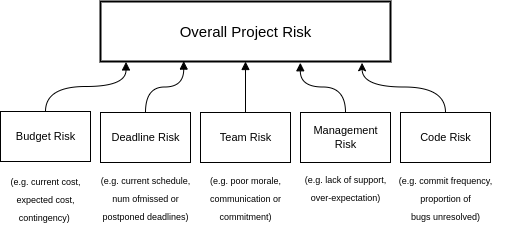
\includegraphics[width=0.9\linewidth]{cr.png} 	
\end{wrapfigure}
Additionally, to meet requirement \textbf{R.4.1}, our system must provide suggestions which can be taken to reduce the risk level, so it is important that the Risk Assessment can be decomposed into components. As such, the model will be divided into five sub-models, each of which provides a risk estimation for a different element of the project (Budget, Deadline, Team, Management and Code). This design offers greater granularity to the Risk-Assessment, so suggestions can be provided according to which component(s) are predicted to fail.
\subsection*{Suggestions}
\begin{wrapfigure}{r}{2.5in}
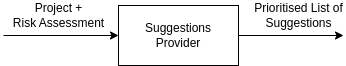
\includegraphics[width=1\linewidth]{arrow.png} 	
\end{wrapfigure}
We have decided that suggestions will be provided by a dedicated SuggestionsProvider object, which takes a Project and its Risk Assessment as input and returns a list of suggestions. The actual implementation will be primitive as it will be hard-coded to return suggestions for each of the five categories which fails in the Risk Assessment. Our main reasoning is that because many projects suffer from similar issues, suggestions can be generic enough to apply to multiple projects.
\subsection*{User Interface}
\begin{figure}[H]
	\centering
	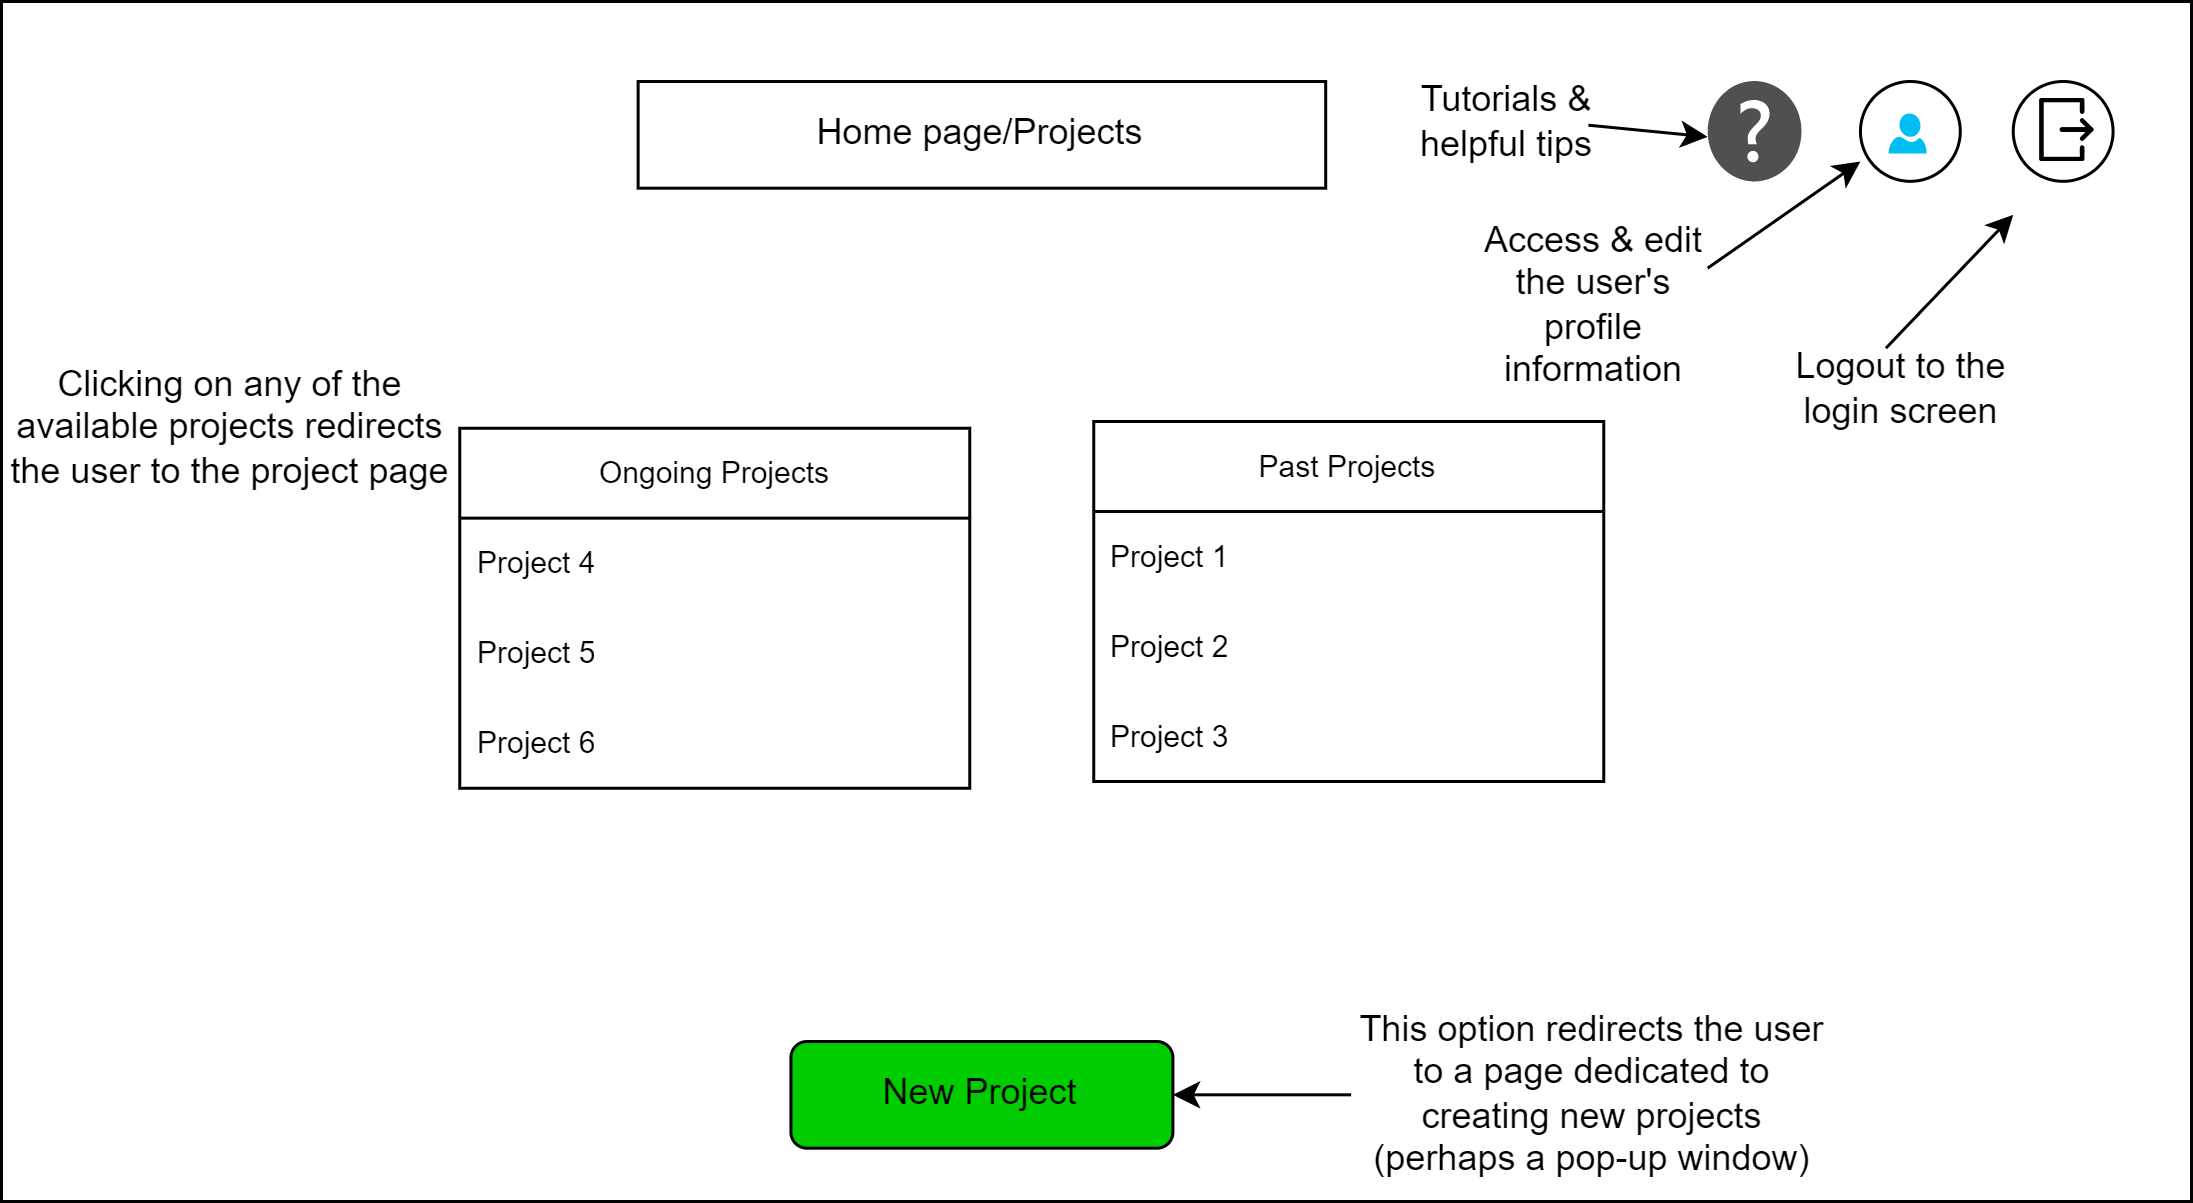
\includegraphics[width=0.9\textwidth]{prm.png}
	\caption{Project Management Interface}
	\label{fig:prm-png}
\end{figure}
This is the design of the home page in which the user may select to view the details of current or past projects
\begin{figure}[H]
	\centering
	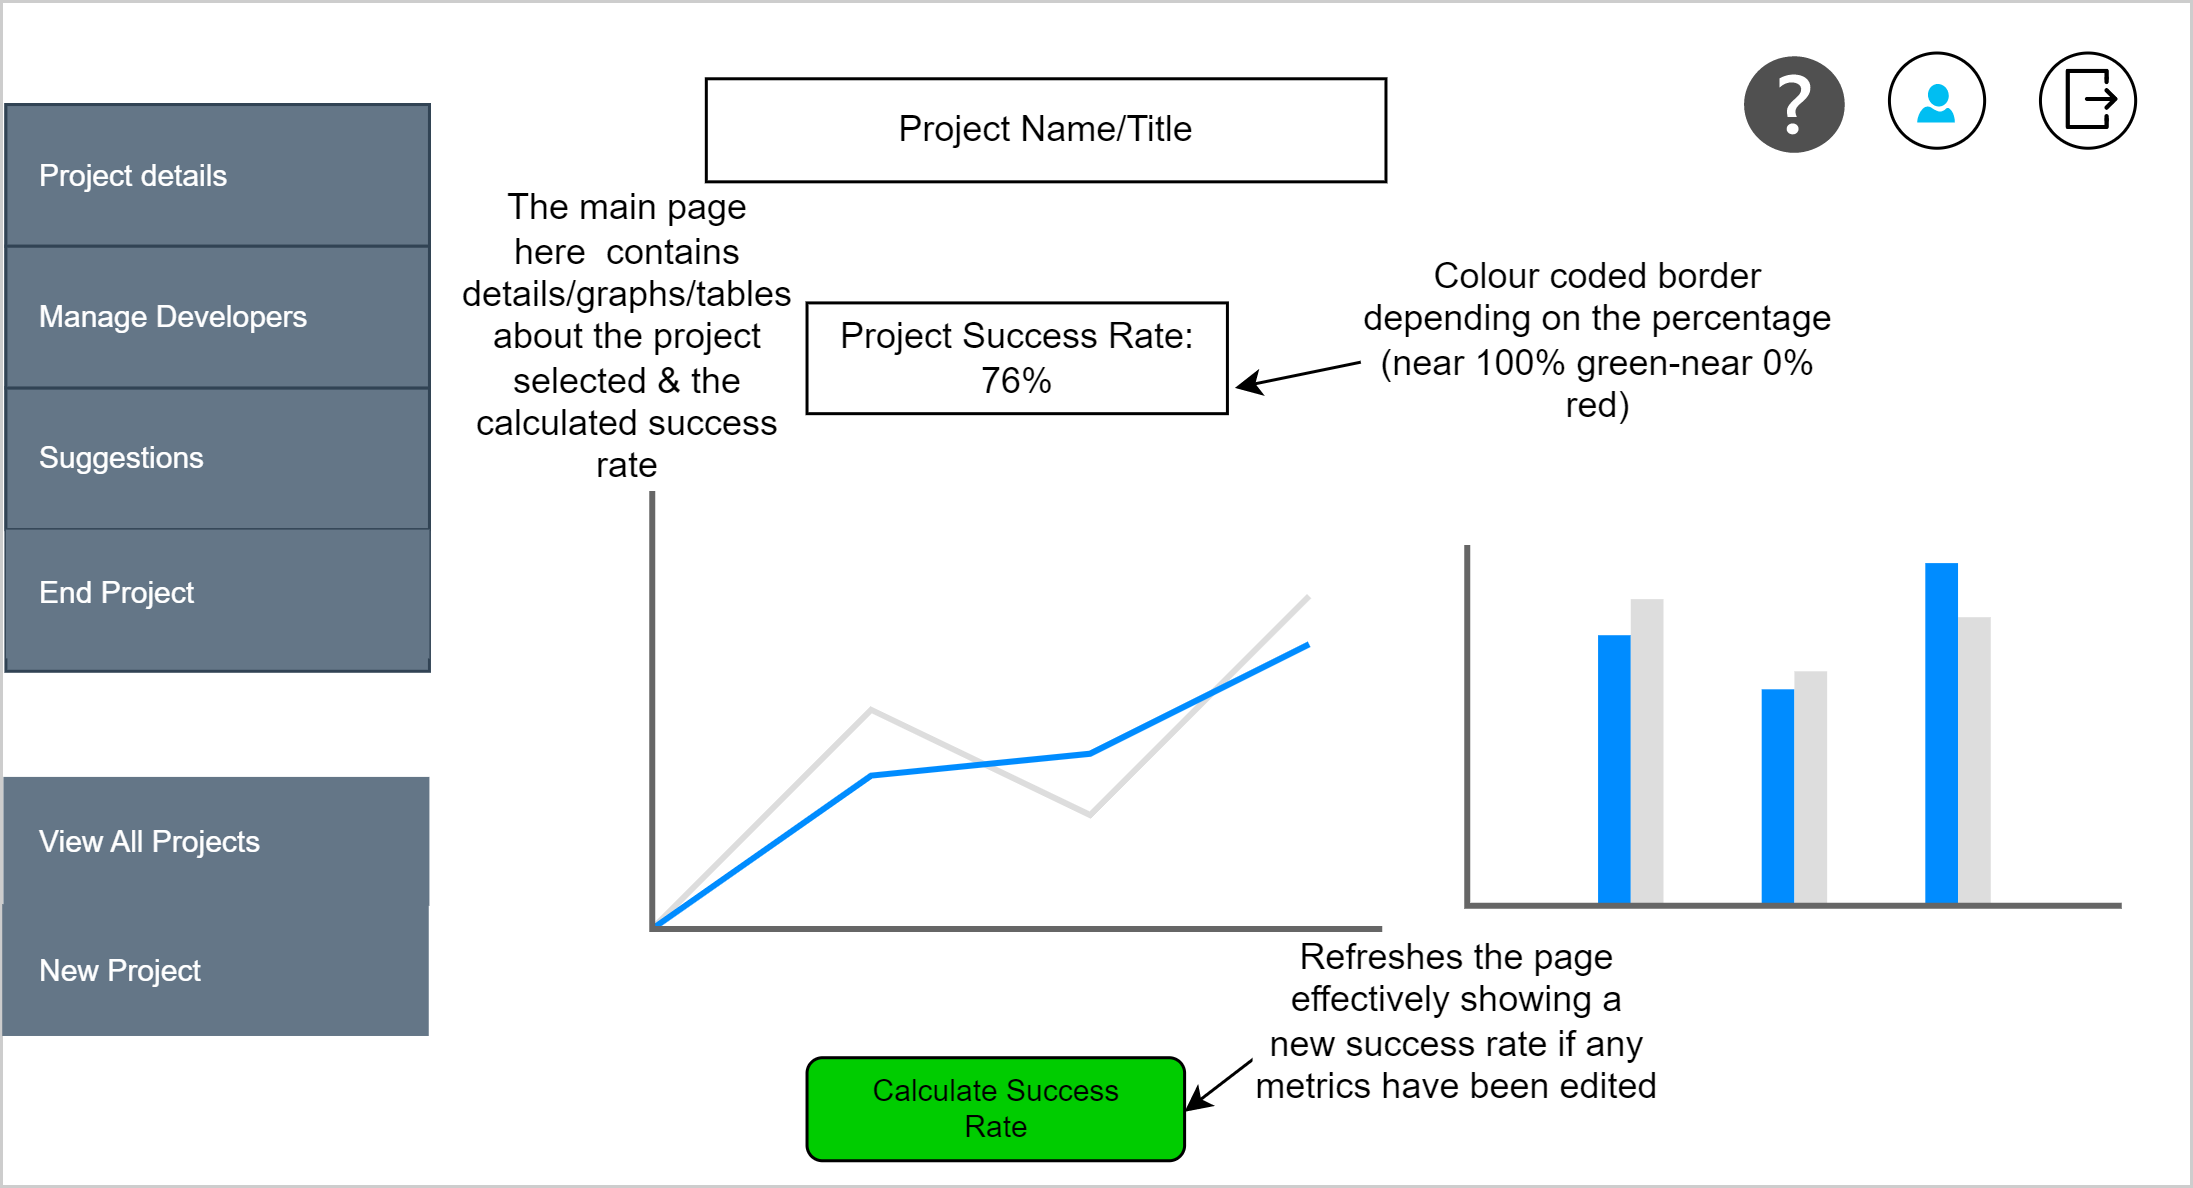
\includegraphics[width=0.9\textwidth]{prs.png}
	\caption{Project Risk and Statistics Page}
	\label{fig:prs-png}
\end{figure}
\noindent Upon clicking on any project, the user is redirected to that project's main page.\\

\noindent The menu provides options through which the user may change the project metrics which should affect the output provided. The output is in the form of tables, graphs, success rate percentages and general suggestions. If any of the metrics have been changed (either from "Manage Developers" or "Project Details" sections), the website automatically refreshes showing updated results. The "Completed" projects will have these modification options greyed out and unclickable, so they cannot be interacted with.
\subsubsection*{UI Design Choices}
The website and the user interface have a concise and minimalist design. It will consist of approximately nine different pages some of which will be represented as pop-up pages or lists. The UI is designed to be clear and have a high affordance to the user using tables, lists and menus wherever possible. Two icons (the account management and the log-out icon) can be found consistently on the top right of every page that supports said features. Additionally, at the bottom of each page there is a button of the same colour that indicates the “interact” button, providing a primary action for that page (e.g. to calculate the success rate, to create a new project or to continue to the next page when choosing which project to interact with). The affordance is provided by the simple icons located in any areas that the user may interact with. In case the user requires assistance, a third icon on the top right of any page that may need it, contains an “information/FAQ” clickable option. Lastly, the main use of the website which is to give suggestions and calculate a success rate of a software project is located in a clear and convenient place within the website so as to minimise user interaction when performing simple tasks.
\subsection*{GitHub}
To provide an effective analysis of the hard code metrics (commit frequency and bug tracking), it was deemed appropriate to link the user’s GitHub repository to our software to access this data. The python library PyGithub contains the necessary functionality to collect information from the user’s specified GitHub repository. A user will need to provide a Personal Access Token, with at least full repo permissions and the URL of the repository in order to successfully sync and extract the required data. Tokens can also be made to expire, so whilst the user should provide a token that will last for the project's duration, deadlines may be altered, and a user will need to provide a token once again.\\

\noindent GitHub has a feature known as GitHub Issues where team members can report any bugs or improvements and mark them as completed when necessary. It also tracks user commits, so the frequency of commits can be extracted. Milestones are another feature of GitHub that let users set deadlines for the project; however since these are not mandated and may not be used by a project, it was deemed appropriate to instead collect this information from the user of our software for reliability.
\section*{Survey}
\subsection*{Survey Questions}
We have determined that measuring soft metrics in our software is necessary to provide an accurate estimation of the project failure risk. Since soft metrics in essence are not quantifiable data, we will collect this data via surveys which contain approximately $5$ questions with a $1$ to $5 $ scale (where $5$ indicates a higher chance of success for all questions, thus standardising the data for the algorithm) to make the metric measurable. The survey will be emailed to all team members to ensure we receive input from all relevant stakeholders. 
\subsection*{Initial Survey}
The initial survey is unique, gathering data from before the software developers have started working on the project. We also require team members to let us know their expertise when they join a project; this is a hard metric, but we take advantage of a survey being sent out to gather this data. \\

\noindent Some examples of survey questions that may be asked (bold indicates the metric being assessed):
\begin{enumerate}
	\item I agree with the initial project requirements $\&$ design planned out by the team - \textbf{Degree of project planning}
\item I fully understand the goals and objectives of the project that the customer is asking for - \textbf{Degree of project planning}
\item Choose the rank which best describes your level of experience as a software developer (\textbf{Hard metric - expertise})
	\begin{itemize}
		\item Rank $1$ - junior software engineer, $1-3$ years, $2+$ languages 
		\item Rank $5$ - senior software engineer, $5+$ years of experience, proficient in most modern languages as well as have other team management skills.
	\end{itemize}
\end{enumerate}
\subsection*{Periodic Survey}
On the other hand, standard surveys will be sent at regular intervals or whenever the manager decides, to the development team to obtain metrics related to the current state of the team. \\

\noindent Some examples of the survey questions would be (bold indicates the metric being assessed):
\begin{enumerate}
	\item I feel that the top management is committed to the success of this project and feel comfortable approaching them with any issues regarding the project - \textbf{Top-level management support}
	\item I feel committed to the success of this project - \textbf{Team commitment}
	\item I feel that the team communicates effectively - \textbf{Team communication}
	\item I am happy and confident working on this project - \textbf{Team Morale}
\end{enumerate}
\subsection*{Frequency of Risk Assessment}
The risk assessment will be calculated after the initial metrics are provided by the manager and the developers. Throughout the duration of the project, the assessment will be recalculated after every change in the data for the project: such as a budget change, or the periodic surveys being completed. If a change occurs, this recalculation will only happen once at $00:00$ GMT. The user is also able to click a button on the website that recalculates the risk and provides new graphical representation and new suggestions (if a change in the risk is present). Alternatively, if no change occurs or no recalculation happens over a certain period of time, the system automatically updates as well. \\

\noindent The reason such limitations are in-place is to ensure the user does not flood the system with high numbers of requests, which would cause multiple database rows to be created for the same date as well as being demanding on our system. 
\subsection*{Visualisation}
\noindent When viewing an ongoing project, users will be presented with the overall risk of failure as well as several graphs presenting the trends for budget, risk and deadlines as mentioned in the requirements. The graphs will be created using the Python library matplotlib.\\

\noindent We decided that plotting every value would be infeasible for long projects which last over hundreds of days, so the system will instead divide the entire project time-frame (from start to deadline) into a fixed number of intervals. For each interval, the system will then plot the highest and lowest value for the risk over that period. This approach will ensure the overall trend is visible, while limiting the resolution of the graph to avoid overwhelming the user.\\

\noindent At the beginning of the project, the graph will be empty as there is no data to plot, but the time frames will already be decided. If a deadline is moved (which is highlighted  in our requirements), then the time frames, and the respective data points will then be recalculated and replotted. This means that a graph that was previously fully-plotted may now be only half full depending on how much the deadline was extended by. \\

\noindent These data visualisation techniques increase the usability of our system and improve the chances that a user will be able to quickly and successfully extract important information about a project. A user is more likely to interact successfully with our website if it presents the risk in a graphical way rather than a text-based way and therefore more likely to come back and use our system again. 

\section*{Testing}
The test plan is laid out according to components of the software (database, user interface etc.) and will be carried out during each sprint cycle ensuring that all components completed during that cycle work as intended.\\

\noindent Initially, we will use preliminary static testing to ensure that the code meets the requirements and to catch any errors. These tests will be performed by other members of the team. Then, we will use Unit-Testing to validate the functionality of specific components and functions, as well as Integration-Testing for interoperability of components (for example, the website login and the database). Given that the majority of the system’s back-end will be written in Python, we will be using the pytest library for unit-testing. Pytest is a well-documented \cite{krekel_2023} test-suite for constructing and running automated tests and is preferable to unittest for the ease with which new test cases can be defined without needing to define a dedicated Test class.
\subsection*{Testing Plan}
\subsubsection*{Database}
Our system’s functionality relies on user and project data being stored and retrieved correctly from the persistent storage (i.e. the SQLite database). We can presume, based on the wide usage of SQLite and its documented testing process \cite{sqlite} that the database integrity will be maintained both between queries and when database operations are interrupted (for example, if power is lost). Therefore, we must focus our tests on ensuring our own SQL Functions, Procedures and Triggers are valid and robust. \\

\noindent For example, consider the function to retrieve the mean value of the soft metrics for a given project over a specific interval: $getMeanProjectResponses(projectID, startDate, endDate)$. We will Unit-Test this function by simulating the contents of the Survey$\_$Response table:
\begin{table}[H]
	\centering
	\caption{Example Survey$\_$Response Test State}
	\label{tab:label}
	\begin{tabular}{|c|c|c|c|c|c|c|c|}
		\hline
		\textbf{Project ID} & \textbf{Worker ID} & \textbf{Date} & \textbf{Metric 1} & \textbf{Metric 2} & \textbf{Metric 3} & \textbf{Metric 4} & \textbf{Metric 5} \\
		\hline
		$11$ & $1 $ &\textbf{ 2020/01/01 }& $4$ & $3$ & $1 $ & $1$ & $1$ \\
		\hline
		$11$ & $2$ & $2020 / 01 / 03$ & $3$ & $3$ & $5$ & $1 $ & $4$ \\
		\hline
		\textbf{12} & $1$ & $2020 / 01 / 03$ & $1$ & $4 $ & $1$ & $5$ & $2$ \\
		\hline
		$11$ & $1 $ & \textbf{2020/01/08} & $2$ & $3$ & $2$ & $4 $ &$1$ \\
		\hline
	\end{tabular}
\end{table}
\noindent Then, we can assert that the expected result for a call with $(projectID=11, startDate=2020/01/01, endDate=2020/01/07)$ will be a tuple of means: $(3.5, 3.0, 1.0, 3.0, 2.5)$, following the same order as the columns in the table above. Notice that to achieve this result, the function must calculate the mean of only the first two rows; essentially, this test verifies four correctness properties:
\begin{enumerate}
	\item The mean of each column is calculated correctly
	\item Row $1$ is \textit{included} (since its date falls on the boundary of the time period)
	\item Row $3$ is \textit{ignored} (since it applies to Project 12, not 11)
	\item Row $4$ is \textit{ignored} (since its date falls outside the time period)
\end{enumerate}
\subsubsection*{Risk Assessment Model}
The Machine-Learning model is difficult to test precisely, since it cannot be expected to produce the correct classification every single time. However, we can require that its performance meets a given accuracy threshold; in particular, we can require that the F-Score \cite{scikit-learn}, a measure of the overall precision and recall, is at least $80\%$. Similarly, sklearn provides methods to generate the Confusion Matrix of the model, which indicates the proportion of mis-classified observations for each pair of classes. 
\subsubsection*{Suggestion System}
\noindent In order to test the Suggestions Provider (SP), we will first need to have fully tested the Risk-Assessment Model (RAM) and validated that its output is appropriate. Then, to test that the Suggestions are selected correctly, we will write a series of Unit-Tests simulating different Risk-Assessment configurations (for example, one project where all categories are successful except for Budget; another project where all are successful except team). For each scenario, the development team will consider the list of suggestions and identify those which are deemed appropriate for the test-case. \\

\noindent Additionally, due to the relationship between the RAM and SP, we will perform Integration-Testing to ensure that both components interact correctly. This will be achieved by designing a series of sample projects and manually identifying appropriate feedback, before feeding each of them into the RAM-SP pipeline one-by-one, and verifying that the returned suggestions are appropriate for the given sample.
\subsubsection*{Website and UI}
\noindent Testing the general functionality of the website is a very high level procedure. A team member other than the person who wrote the front end code will attempt to input erroneous data as well as navigate the website in “unorthodox” ways. Some such ways could be to log out of an account and then press the “back” button on the top left of the browser, attempting to log back in that way. Another detail of the website mentioned in requirement \textbf{R.1.2}, i.e., logging a user out from an older device when the same user attempts logging in from a new device, can be trivially tested.\\

\noindent Usability testing will also be carried out by non-technical users. These acceptance tests will highlight the ways in which different users may perceive web-page elements. Non-technical users will be asked to complete a series of tasks and later asked to review how they felt using the website. This ensures that the website is built in such a way that is usable and easy to understand for all users despite having different technical capabilities, fulfilling requirement \textbf{R.5.1}.\\

\noindent Static UI tests will be performed to ensure that all features work as it is intended. For example, the usage of the “question mark” icon will be tested to ensure that it is able to guide non-technical users to be able to use the website with minimal training and works as intended, ensuring that requirement \textbf{R.5.3} is met.\\

\noindent As mentioned in requirement \textbf{R.5.4}, we will mainly test the website on Google Chrome version 109.0.5414.119 on Windows 10. However, the website should be compatible with any other browser that supports Bootstrap 5 and its respective Javascript version. Testing this will be a matter of running the website on different browsers (for example, Firefox, Safari, Microsoft Edge) and using the features of the interface that use Bootstrap or interact with JS. Any observations will be well-documented.\\

\noindent We will also be testing how the website renders on different screen sizes such as mobile phones and laptops to check requirement \textbf{R.5.5}. Load testing will be carried out where different scenarios are stimulated to check the behaviour of the system under different throughput by the user to ensure requirement \textbf{R.5.6} is fulfilled.
\subsubsection*{GitHub Linkage}
To ensure our software receives the correct information regarding the project's code, it is important to check if our software successfully obtains this data (\textbf{R.2.2}). By setting up a sample repository, we can perform unit tests between our software and the repository such as:
\begin{itemize}
	\item After opening nine issues, each with one of the $9$ different labels, run the $open\_issues\_count()$ function to check all issues are being detected
	\item Using $get\_issues(state=’open’)$, iterate through all results and display them, comparing them against the issues open in the repository and check they are identical
	\item Set the repository to Private, and check the provided token still has access to the repository 
\end{itemize}
\section*{Process Documentation and Risk Assessment}
We have chosen an Agile methodology, inspired by Scrum. Due to the nature of our development, we do not have full access to the client and so we could not fully implement Scrum. We have chosen to enact weekly cycles, each following these steps: sprint planning, the sprint, and the sprint review. An initial product backlog, consisting of the components necessary to the software has been constructed. This will evolve as the project progresses as more information is gathered about how the team works best and any further functionality the software may need. During sprint planning, this backlog will have the most pressing items taken from the stack (for example, establishing the database is crucial as many future components will interact with it) and broken down into sub-tasks that can be feasibly completed in a cycle, such as the production of a schema, or the database triggers. Each task also requires testing so these will also be allocated in the cycle to be designed and implemented. Once the plan is agreed upon, the sprint can begin, in which each team member works to complete their allotted tasks. To ensure progress is made, daily scrum meetings will be held to track everyone’s progress and ensure the tasks are completed by the end of the cycle. Once a cycle is finished, all completed tasks can be removed from the product backlog. Finally, the review is when all the team members can demonstrate their work to the rest of the team, and any comments and improvements can be added to the backlog to be addressed in the following cycle. In order to promote the smooth completion of cycles, we have elected a Scrum-Master who will be responsible for leading the sprint meetings (planning, daily and review). \\

\noindent The following is an outline of what each cycle hopes to address, but as each cycle progresses, these events will naturally be broken down further and completed at different rates as some subsystems are more complex than others:
\begin{figure}[H]
	\centering
	\includegraphics[width=0.8\textwidth]{Gantt.jpeg}
	\caption{Cycle Gantt Chart}
	\label{fig:cgc}
\end{figure}
\subsection*{Risks}
Risks have been ordered by decreasing potential impact to the development. The inherent risk refers to the threat-level posed when no effort is made to mitigate the danger whereas residual risk is the remaining threat after a treatment has been put into place. We also provide an explanation of how each risk applies to our team \cite{wilson_2022}.
\begin{table}[H]
\begin{tabular}{|c|c|c|c|c|c|}
\hline
\rowcolor[HTML]{C0C0C0}
\textbf{Risk}                                                                                           & \textbf{Summary}                                                                                                                                                 & \textbf{\begin{tabular}[c]{@{}c@{}}Inherent\\ Risk\end{tabular}} & \textbf{Treatment}                                                                                                                                                                                                 & \textbf{\begin{tabular}[c]{@{}c@{}}Residual\\ Risk\end{tabular}} & \textbf{Explanation}                                                                                                                                                                                                                                                                                                                       \\ \hline
\begin{tabular}[c]{@{}c@{}}Size\\ Underestimate\\ or timescale\\ not estimated\\ correctly\end{tabular} & \begin{tabular}[c]{@{}c@{}}Underestimating the\\  complexity of the\\  project and requirements\\ which creates a risk of\\ going over the deadline\end{tabular} & \cellcolor[HTML]{E06666}High                                     & \begin{tabular}[c]{@{}c@{}}Ensure a clear timeline\\ is developed over time,\\ with each task broken\\ down into manageable\\ sub sections that are\\ understood by\\ everyone\end{tabular}                        & \cellcolor[HTML]{F6B26B}Medium                                   & \begin{tabular}[c]{@{}c@{}}Due to our minimal\\  experience with \\ projects of this size,\\  it is hard for us to\\  reliably estimate the\\  complexity and time-\\ scale correctly. \\ However, we have\\  focused on designing\\  a system which can\\  be implemented with\\  the knowledge and\\  tools available to us\end{tabular} \\ \hline
\begin{tabular}[c]{@{}c@{}}Not completing\\ cycle(s) on time\end{tabular}                               & \begin{tabular}[c]{@{}c@{}}If the end of the cycle(s)\\  is reached without\\  finishing all the tasks out-\\ lined in the cycle timeline\end{tabular}           & \cellcolor[HTML]{E06666}High                                     & \begin{tabular}[c]{@{}c@{}}Have a member of the \\ team assigned to track\\  the progress of each\\  cycle and ensure all\\  the developers are\\  completing the tasks\end{tabular}                               & \cellcolor[HTML]{F6B26B}Medium                                   & \begin{tabular}[c]{@{}c@{}}As students, we are \\ not developing the\\ program full-time \\ and therefore can\\  fall behind on the\\  plan we have set out\end{tabular}                                                                                                                                                                   \\ \hline
\begin{tabular}[c]{@{}c@{}}Tool\\ Underperformance\end{tabular}                                         & \begin{tabular}[c]{@{}c@{}}Libraries or software we\\  intend to use are not\\  performing the way\\  it was expected.\end{tabular}                              & \cellcolor[HTML]{F6B26B}Medium                                   & \begin{tabular}[c]{@{}c@{}}Perform appropriate re-\\ search before intro-\\ ducing new tools.\\  This should happen\\  in the design stage\\  of the project.\end{tabular}                                         & \cellcolor[HTML]{93C47D}Low                                      &                                                                                                                                                                                                                                                                                                                                            \\ \hline
\end{tabular}
\end{table}
\begin{table}[H]
\begin{tabular}{|c|c|c|c|c|c|}
	\hline
\begin{tabular}[c]{@{}c@{}}Specification\\  delays/ change in\\  requirements\end{tabular}              & \begin{tabular}[c]{@{}c@{}}The client not presenting\\  the specification in\\  time or requirements \\ are constantly changing.\end{tabular}                    & \cellcolor[HTML]{93C47D}Low                                      & \begin{tabular}[c]{@{}c@{}}The agile methodology\\  we have chosen allows\\  us to assess new \\ requirements at the\\  beginning of each\\  cycle and decide if\\  implementing them\\  is feasible.\end{tabular} & \cellcolor[HTML]{93C47D}Low                                      & \begin{tabular}[c]{@{}c@{}}The client has already\\  presented the specifi-\\ cation to us. There is\\  a chance we will\\  change our re-\\ quirements as we\\  start development\\  however this can\\  be planned for at\\  the beginning of\\  each cycle.\end{tabular}                                                                \\ \hline
\begin{tabular}[c]{@{}c@{}}Change in group\\  members\end{tabular}                                      & \begin{tabular}[c]{@{}c@{}}Team members leaving\\  the group and a new\\  person joining who is\\  unaware of the aims \\ of the project.\end{tabular}           & \cellcolor[HTML]{93C47D}Low                                      & \begin{tabular}[c]{@{}c@{}}Re-allocate the roles\\  such that at least two\\  people are responsible\\  for each component.\end{tabular}                                                                           & \cellcolor[HTML]{93C47D}Low                                      & \begin{tabular}[c]{@{}c@{}}If any team member\\ leaves, for example in\\  our case if someone\\  drops the module or\\  leaves the university;\\  we will have redun-\\ dancy in the form of\\  at least one other mem-\\ ber able to work on\\  each feature and\\  explain the re-\\ quirements to a\\  new member.\end{tabular}         \\ \hline
\end{tabular}
\end{table}
\noindent Overall, we believe that the risk of our project is manageable; we should be able to complete all the tasks, and meet the requirements if we plan for the risks and work towards mitigating them as outlined in the table. During each weekly meeting, we will continue to reassess the risks and ensure that any issues are managed correctly.
\bibliographystyle{apacite}
\bibliography{bibliography}
\end{document}
